%%%%%%%%%%%%%%%%%%%%%%%%%%%%%%%%%%%%%%%%%%%%%%%%%%%%%%%%%%%%%%%%%%%%
% Overivew
%%%%%%%%%%%%%%%%%%%%%%%%%%%%%%%%%%%%%%%%%%%%%%%%%%%%%%%%%%%%%%%%%%%%

\begin{algorithm}[!t]
	\caption{Algorithm to design an interlocking assembly $\mathbf{A}_n$ from a given shape $R_0$.}
	\begin{algorithmic}[1]
		\Function{CreateInterlockAssembly}{$R_0$}

		\State $i \gets 0$
		\State $A_i^{*} \gets [R_0]$
				
		\While {$i < n$} 
		\If{ $i$=0}
		\State{$\{A_{i+1} \}$  $\gets$ GenerateKey($A_i^{*}$)	}  \Comment{See Subsection~\ref{subsec:genKey}}
		\If{$\{A_{i+1} \} = \emptyset$}
		\State   \Return NULL 
		\EndIf
		
		\Else
		\State $\{A_{i+1} \}$ $\gets$ GenerateParts($A_i^{*}$)  \Comment{See Subsection~\ref{subsec:genPart}}
		\EndIf
		
		\vspace{1.0mm}
		\If{$\{A_{i+1} \} \neq \emptyset$}
		\State RankCandidates($\{A_{i+1} \}$)     \Comment{In descending order}   % { i.e., $A_{i+1}^1$ is the best one }
		\If{ $i+1 =  n$}
		\State   \Return $A_n^1$				
		\Else
		\State 	$i \gets i+1$  
		\State $A_i^{*} \gets A_{i}^1$ 
		\EndIf
		
		\ElsIf{$A_i^{*}.sibling \neq NULL$}  
		\State	$A_i^{*} \gets A_i^{*}.sibling$   \Comment{$A_i^{*}.sibling$ is the one second to $A_i^{*}$ in the ranked $\{A_{i} \}$}
		
		\Else
		\While{$A_i^{*}.parent \neq$ NULL $\&\&$  \\  \hspace{22.0mm}   $A_i^{*}.parent.sibling =$ NULL}
		\State	$A_i^* \gets A_i^{*}.parent$ 
		\State $i \gets i-1$
		\If {$i= 0$}   \Comment{Quit if backtrack to $A_0$  }
		\State{\Return NULL}
		\EndIf
		\EndWhile
		
		\If {$A_i^{*}.parent \neq$ NULL $\&\&$ \\ \hspace{17.0mm} $A_i^{*}.parent.sibling  \neq$ NULL}
		\State $A_i^* \gets A^*.parent.sibling$			
		\Else      
		\State	\Return NULL 
		\EndIf
		
		\EndIf
		
		\EndWhile
		
		\EndFunction
	\end{algorithmic}
	\label{alg:Alg_Framework}
\end{algorithm}

\section{Computational Design Framework}
\label{sec:approach}

%%%%%%%%%%%%%%%%%%%%%%%%%%%%%%%%%%%%%%%%%%%%%%%%
% Problem Formulation
%%%%%%%%%%%%%%%%%%%%%%%%%%%%%%%%%%%%%%%%%%%%%%%%

%\Mark{I think this section needs an overview first. Below we describe an iterative procedure that could fail at several locations. But we do not describe what happens in such a case. Do we back-track? Start over? How do we avoid making bad decisions early on whose consequences will only become apparent much later?
%What can we say about the outcome of the method. If it doesn't find a solution, can we guarantee that none exits? Or in other words, if a solution exists, are we guaranteed to find it? We should probably explain upfront the two-stage approach and motivate why it makes sense, but also mention what the drawbacks are.}

%\vspace*{1.0mm}
%\noindent
%{\bf Problem Formulation.}  \
Given our efficient algorithm to test for interlocking, our main goal is now to provide effective algorithms for designing interlocking assemblies. We first provide a high-level overview of our framework before presenting the conceptual and algorithmic details.

As input we expect the final shape of the assembly, from which the component parts are either constructed from scratch as in~\cite{Xin-2011-BurrPuzzles, Song-2012-InterCubes,Song-2015-Interlock} or explicitly initialized as in~\cite{Fu-2015-Furniture, Song-2016-CoFiFab,Yao-2017-InterlockShell}.
%Requirements on the geometry of the parts (e.g., for fabrication) and/or the final assembly (e.g., aesthetics) may need to be considered in the design process, depending on the application.
%
%For the latter case, the neighboring relationship among the parts have been given, which define the set of part pairs for constructing blocking relations. 
Our computational process for creating an interlocking assembly starts with the full input model, then iteratively splits off successive parts for disassembly. At each iteration, we first identify a set of suitable blocking relations between the current assembly and the new part to be generated such that the interlocking property is maintained. Then we search for the part geometry that satisfies these blocking relations. The selection of a new part is guided by a ranking function that takes into account certain geometric properties, e.g. part size, or other requirements, e.g. on part fabrication.
The search space is then explored in a tree traversal process that uses automatic backtracking when no interlocking solution could be found in a specific iteration. We also provide a user interface to interactively explore different options for part decomposition, allowing the user to  overwrite the generic ranking function for part selection.



%%%%%%%%%%%%%%%%%%%%%%%%%%%%%%%%%%%%%%%%%%%%%%%%
% Iterative Design Framework
%%%%%%%%%%%%%%%%%%%%%%%%%%%%%%%%%%%%%%%%%%%%%%%%

\subsection{Iterative Design Framework}
\label{subsec:framework}

%\vspace*{1.0mm}
%\noindent
%{\bf Iterative Design Framework.}  \
Given the input shape denoted as $R_0$, we iteratively construct the geometry of each part (or introduce appropriate joints in the geometry of each initialized part; see Section~\ref{subsec:furniture}), one by one. This forms a sequence of constructed parts, $P_1$, $P_2$, $...$, $P_n$, with $R_n$, the remaining part of $R_0$, as the last part:
%In other words, we iteratively partition remaining part $R_{i-1}$ into two parts to form $P_i$ and $R_i$:
\begin{displaymath}
[R_0] \rightarrow [P_1,R_1] \rightarrow [P_1,P_2,R_2] \rightarrow ... \rightarrow [P_1,...P_n,R_n] \ .
\end{displaymath}
Here we denote each intermediate assembly $[P_1, ..., P_i, R_i]$ as $\mathbf{A}_{i}$ ($0 \leq i \leq n$), and its base DBGs as $\{ G(d, A_i) \}$. 
Figure~\ref{fig:Framework_Overview} shows an example where the parts are constructed from scratch.


%When parts have been initialized, we consider all those untouched parts as $R_{i-1}$ ($i\geq1$) conceptually when constructing $P_i$ and $R_i$ from it. 
%\Peng{Would it be sufficient to guarantee interlocking by constructing a single piece at a time; e.g., shall we construct a few pieces together for furniture?}

% Requirements on the construction of $P_i$ and $R_i$
To guarantee that the resulting assembly $\mathbf{A}_n = [P_1, ..., P_n, R_n]$ is interlocking and disassemblable, we have the following requirements when decomposing $R_{i-1}$ into $P_i$ and $R_i$:
\begin{enumerate}[label=(\roman*), leftmargin=*]
	\vspace*{-0.5mm}
	\item
	{\em  Connected.} \
   The geometries of $P_i$ and $R_i$ should each be simply connected, making $\mathbf{A}_i$ a valid assembly. 
   
   	\vspace*{0.5mm}
    \item
   {\em Interlocking.} \
   $\mathbf{A}_i$ ($i\geq2$) is interlocking with $P_1$ as the key.
   In other words, $\{G(d, A_i)\}$ should satisfy the interlocking requirement described in Section~\ref{sec:model}.
   %This is achieved by constructing the geometry of $P_i$ and $R_i$ to satisfy the two interlocking requirements on $\{G(d, A_i)\}$. 

   	\vspace*{0.5mm}
   	\item
   	{\em Disassemblable.} \
   	$P_i$ can be removed from $[P_i, R_i]$, so we can disassemble $\mathbf{A}_i$ in the order of construction $P_1$, $P_2$,  $...$,  $P_i$, $R_i$.
   	
	%try to find the fewest internal blocking relations to be constructed between $P_i$ and $R_i$ such that the strongly connected property is preserved; see Figure~\ref{fig:Framework_Conceptual}(d).
	%This is because fewer internal blocking relations provide more flexibility to construct the geometry of $P_i$ and $R_i$.	
\end{enumerate}	
\vspace*{-0.5mm}
\noindent
The advantage of this iterative design framework is that we achieve the goal of global interlocking by satisfying a set of local requirements when constructing each pair of $P_i$ and $R_i$.

\vspace*{1.0mm}
\noindent
{\bf Tree Traversal.}  \
Since we cannot guarantee that the construction of $P_i$ and $R_i$ succeeds at every iteration, we propose an iterative approach with backtracking to construct $\mathbf{A}_n$; see Figure~\ref{fig:Framework_Overview} and Algorithm~\ref{alg:Alg_Framework}.
The key idea is to build and maintain a construction tree, where each node represents a candidate of $\mathbf{A}_i$. For each node we generate a set of children denoted as $\{\mathbf{A}_{i+1}\}$. 
% by generating a set of $\mathbf{A}_{i+1}$ denoted as $\{\mathbf{A}_{i+1}\}$ from $\mathbf{A}_{i}$ at each iteration.
% by trying different ways of partitioning $R_{i-1}$ into $P_i$ and $R_i$.
Our approach ranks these candidate assemblies at each iteration to facilitate the construction of successive parts.
For example, we rank $\{\mathbf{A}_{i+1}\}$ according to the compactness of $R_{i+1}$, since parts extracted from a compact $R_{i+1}$ are more likely to be simply connected; compare $R_1$ in Figure~\ref{fig:Framework_Overview}(c\&f). 
In case the user has other design goals besides interlocking, e.g., regarding the appearance of the assembly, we support user intervention to adjust the ranking.
%
In case we cannot generate any valid result from the selected candidate in $\{\mathbf{A}_{i+1}\}$, we can backtrack the tree to try other nodes without restarting the whole design process.
The size of $\{\mathbf{A}_{i+1}\}$ is denoted as $M$.
A large $M$ requires more time for generating $\{\mathbf{A}_{i+1}\}$, but also provides more choices for ranking and backtracking. We set $M = 30$ by default in our experiments but it can be adjusted, depending on the input model. 

%In case users have other requirements on the assembly besides interlocking (e.g., appearance), our framework supports user intervention to adjust the ranking.}
%\Mark{We should have a forward reference to an example of user intervention. In general, right now it remains abstract what exactly the ranking function is.}
%\Peng{Text has been revised accordingly.}

%Our framework cannot guarantee to find a solution if it exists, nor guarantee non exists if we cannot find any solution.
%These questions can be answered by exhaustive search only in very small scale design problems; see the experiment in Section~\ref{sec:results}.
%The usefulness of our framework is to provide general computational support for users to design interlocking assemblies according to their desires, which is extremely challenging for manual effort.
Below we explain our approach to generate the key part (Subsection~\ref{subsec:genKey}) and the remaining parts of the assembly (Subsection~\ref{subsec:genPart}). These steps can be customized to design different kinds of interlocking assemblies as discussed in Section~\ref{sec:results}.
Here, we take 2D interlocking puzzle design as an example for illustration.



%Thanks to the DBG-based representation, we can test and further guarantee interlocking for each intermediate assembly $\mathbf{A}_i$ efficiently. %which is previous works~\cite{Song-2012-InterCubes,Fu-2015-Furniture} intentionally skip this step due to the exponential complexity of their interlocking testing algorithm.



%which is achieved by performing the DBG-based interlocking test described in Section~\ref{sec:model}. 
%Note that this interlocking test is intentionally skipped by previous works~\cite{Song-2012-InterCubes,Fu-2015-Furniture} due to their exponential complexity of brute-force search.
%Lastly, we ensure that $A_i$ is disassemblable by requiring $P_j$ to be separable from $R_j$ for every pair of $[P_j, R_j]$, where $1 \leq j \leq i$.
%By this, we guarantee that the resulted assembly $A_n = [P_1, ..., P_n, R_n]$ is interlocking and disassemblable.


\begin{figure*}[!t]
	\centering
	%\vspace*{-3.5mm}
	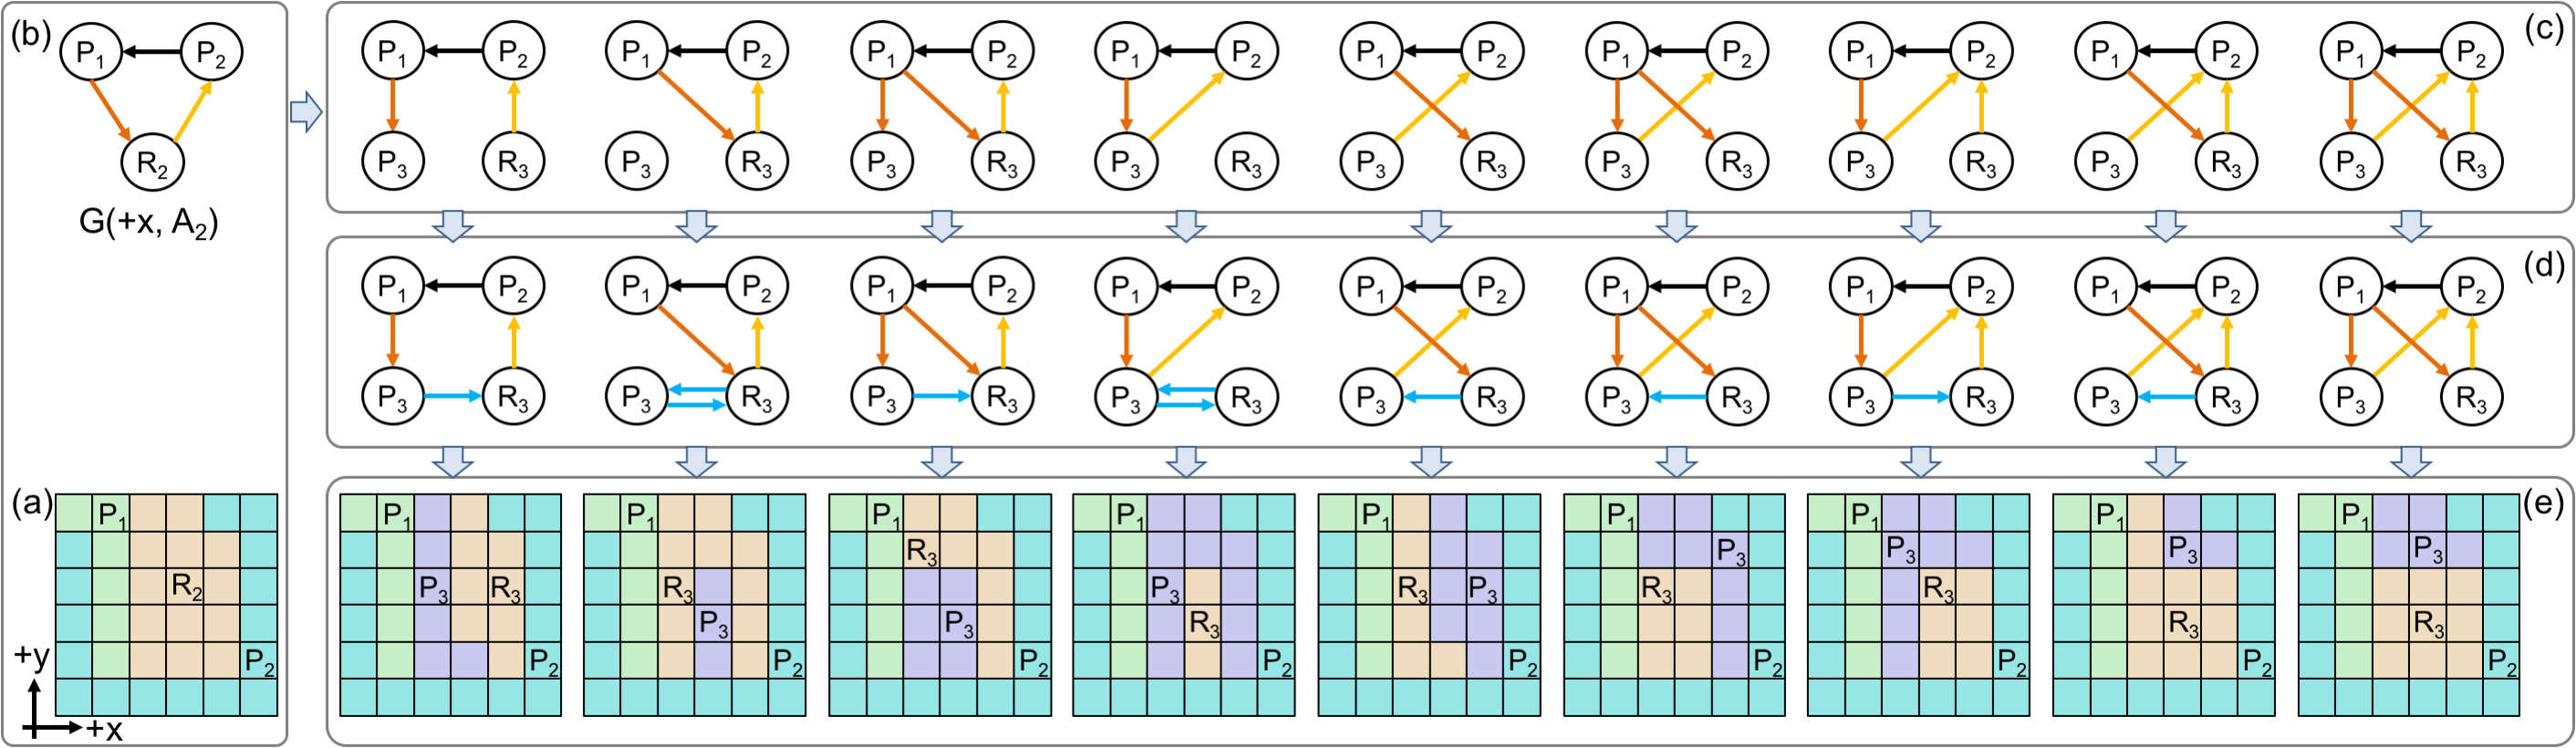
\includegraphics[width=17.80cm]{images/Framework_Conceptual.png}
	\vspace*{-2.5mm}
	\caption{
		(a) An intermediate assembly $\mathbf{A}_2$ and 
		(b) its base DBG $G(+x, A_2)$, where the in-edge and out-edge of $R_2$ are colored in dark and light orange respectively;
		(c) all cases of distributing existing blocking relations (dark and light orange edges) to $P_3$ and $R_3$; 
		(d) the interlocking graph designs that require the fewest internal blocking relations (blue edges) between $P_3$ and $R_3$; and
		(e) the corresponding geometric examples.
	}
	\vspace*{-1.0mm}
	\label{fig:Framework_Conceptual}
\end{figure*}

\begin{figure*}[!t]
	\centering
	%\vspace*{-3.5mm}
	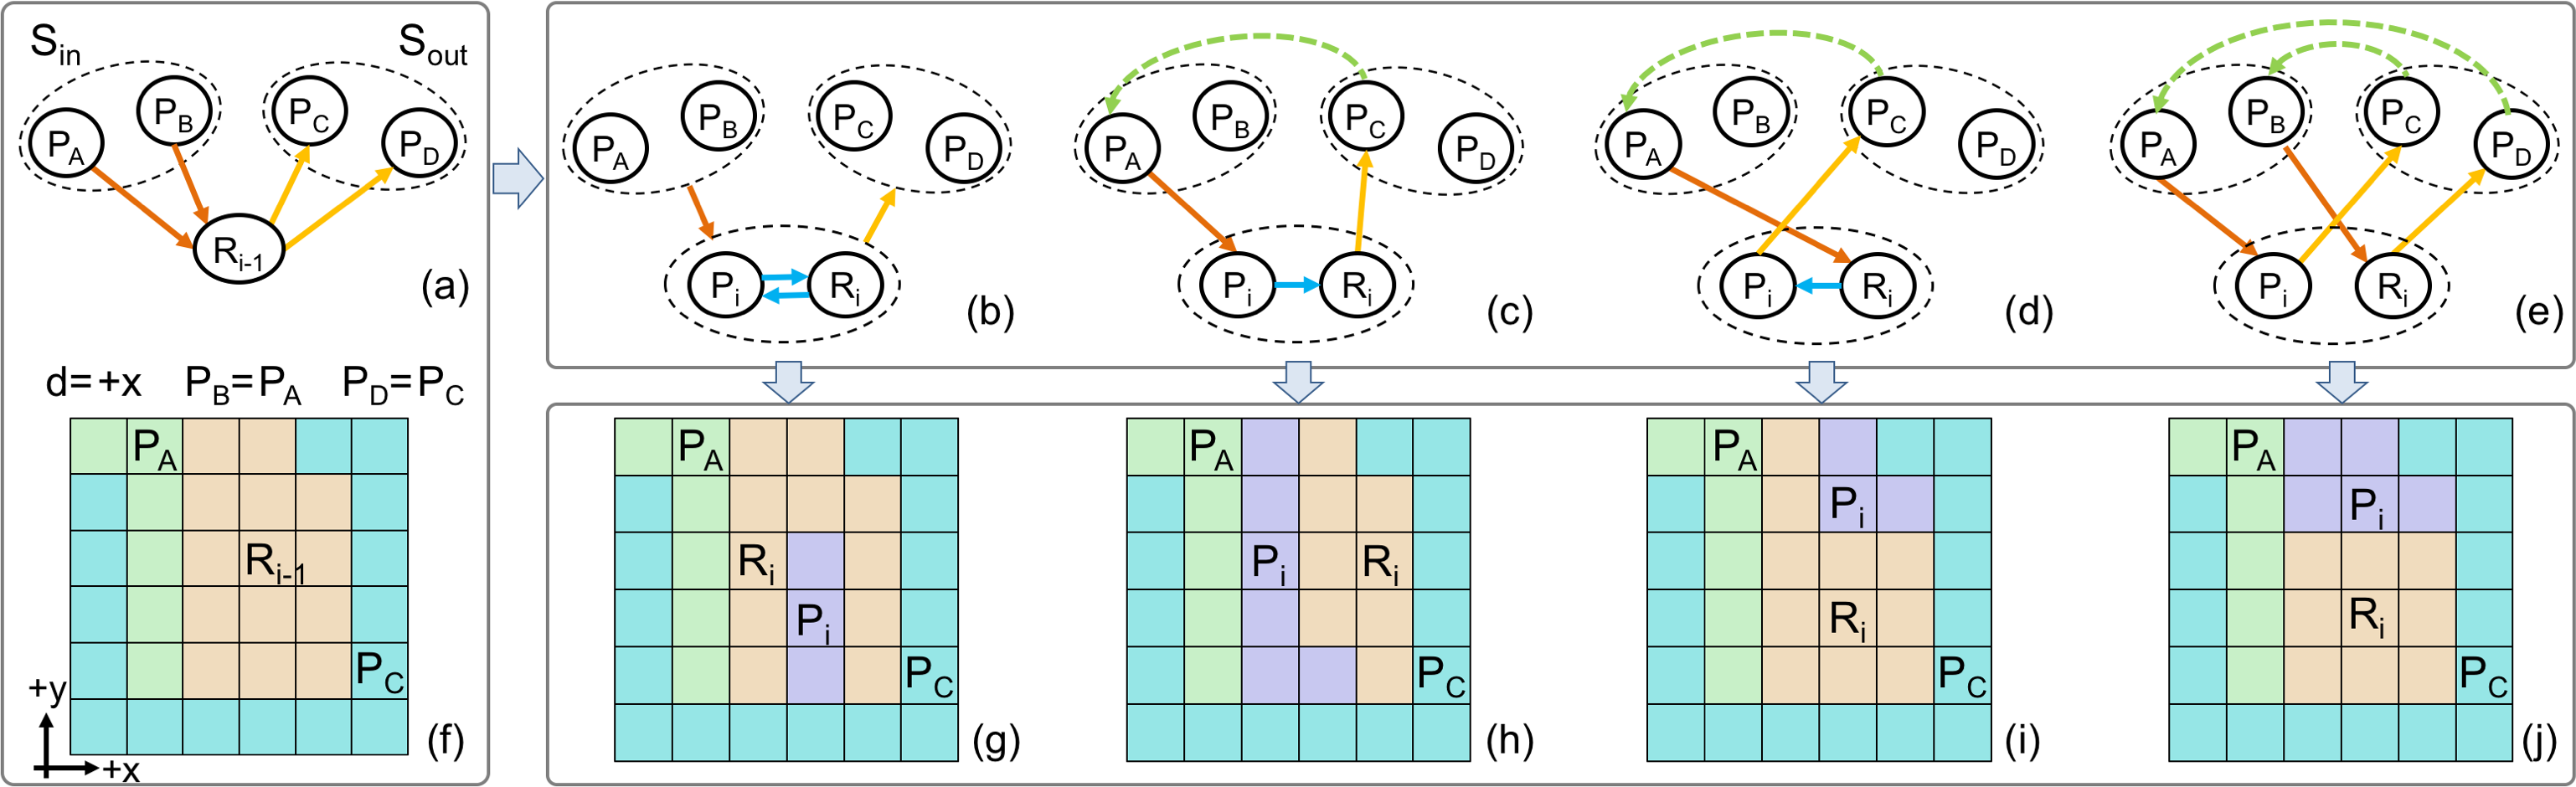
\includegraphics[width=14.50cm]{images/Framework_Cycle.png}
	\vspace*{-2.5mm}
	\caption{
		(a) Given $G(d, A_{i-1})$, (b-e) we ensure that $G(d, A_i)$ is strongly connected by constructing a cycle that includes both $P_i$ and $R_i$.
		A dashed ellipse in (a-e) indicates a subset of parts, i.e., $S_{in}$, $S_{out}$, and $\{P_i, R_i\}$, where $S_{in}$ ($S_{out}$) denotes the set of parts with an edge to (from) $R_{i-1}$.
		The directed edges from (to) a dashed circle in (b) indicate that the edge can be from (to) any part in the associated subset.
		The dashed green edges in (c-e) indicate that a part can reach the other part in $G(d, A_{i-1})$ without passing through $R_{i-1}$.
		(f-i) Geometric examples corresponding to (a-e), where $d = +x$, $S_{in} = \{P_A\}$, and $S_{out} = \{P_C\}$.
		%\Mark{I find this figure confusing. We have $P_A$, etc. in the top row, but below we show something different, i.e. $P_1$. Can't we find an example that is consistent? We should probably also specify $d$.}
		%\Peng{The symbols have been revised in the figure. I have spent an hour in trying to design a more complex 2D example with 6 pieces but failed. Such a example that shows all four cases together seems not easy to find.}
	}
	\vspace*{-2.5mm}
	\label{fig:Framework_Cycle}
\end{figure*}



%%%%%%%%%%%%%%%%%%%%%%%%%%%%%%%%%%%%%%%%%%%%%%%%
% Generate P_1 and R_1
%%%%%%%%%%%%%%%%%%%%%%%%%%%%%%%%%%%%%%%%%%%%%%%%

\vspace*{-0.8mm}
\subsection{Generating the key}
\label{subsec:genKey}

We first partition the input model $R_0$ into $P_1$ and $R_1$, where $P_1$ is the key and $R_1$ is the remaining part.
We construct the geometry of $P_1$ following the procedure in~\cite{Song-2012-InterCubes}; i.e., select a seed pixel, ensure its blocking and mobility, and expand the key piece.
Recall that the key is the only movable (thus unstable) part in an interlocking assembly.
Therefore, we restrict $P_1$ to have a single movable direction in $\mathbf{A}_1$ denoted as $d_1$, and usually select $d_1$ being upward to stabilize $P_1$ with gravity; see Figure~\ref{fig:Framework_Overview}(b\&c) for two examples.
We rank the candidates in $\{\mathbf{A}_1\}$ according to the compactness of $R_1$.
% since more compact $R_1$ will encourage generation of successive parts. 


%%%%%%%%%%%%%%%%%%%%%%%%%%%%%%%%%%%%%%%%%%%%%%%%
% Generate P_i and R_i
%%%%%%%%%%%%%%%%%%%%%%%%%%%%%%%%%%%%%%%%%%%%%%%%

\vspace*{-0.8mm}
\subsection{Generating $P_i$ and $R_i$ $(i>1)$} 
\label{subsec:genPart}
Next, we construct $P_i$ and $R_i$ from $R_{i-1}$ in two stages: {\em graph design} and {\em geometry realization}.
The first stage constructs base DBGs $\{G(d, A_i)\}$ that satisfy the interlocking requirement conceptually while the second stage aims at realizing the blocking relations described in $\{G(d, A_i)\}$ in the embedded geometry.
Note that geometric constraints (e.g., supported joint types) can be used to simplify graph design by eliminating  potential graph edges that cannot be realized geometrically anyway.


%%%%%%%%%%%%%%%%%%%%%%%%%%%
% Conceptual Design of P_i and R_i
%%%%%%%%%%%%%%%%%%%%%%%%%%%

\vspace*{1.0mm}
\noindent
{\bf Graph Design for $P_i$ and $R_i$.}  \
Starting from $\mathbf{A}_{i-1}$ ($i \geq 2$),  the goal is to find blocking relations for $P_i$ and $R_i$  such that the updated assembly $\mathbf{A}_{i}$ is still interlocking.
In other words, after splitting $R_{i-1}$ into $P_i$ and $R_i$ in $\{G(d, A_{i-1})\}$ to form $\{G(d, A_i)\}$, we need to construct a set of new edges of $P_i$ and $R_i$ in each $G(d, A_i)$ such that the graph remains strongly connected, except the key; see Figure~\ref{fig:Framework_Overview}.
To achieve this goal, we first classify blocking relations to be constructed into two classes:
\begin{enumerate}[label=(\roman*), leftmargin=*]
	\vspace*{-0.5mm}
	\item
	{\em External blocking relations} between $\{P_1, ..., P_{i-1}\}$ and $P_i$, as well as those between $\{P_1, ..., P_{i-1}\}$ and $R_i$ are inherited from those between  $\{P_1, ..., P_{i-1}\}$ and $R_{i-1}$.
	Thus, we need to distribute these existing blocking relations to $P_i$ and $R_i$; see Figure~\ref{fig:Framework_Conceptual}(c).
	
	\vspace*{0.5mm}
	\item
	{\em Internal blocking relations} between $P_i$ and $R_i$.
	For each case of distribution of external blocking relations, we may need to construct internal blocking relations between $P_i$ and $R_i$ such that each $G(d, A_i)$ remains strongly connected\footnote
	{If the key is movable along $d$, $G(d, A_i)$ is strongly connected without considering the key. Otherwise, the whole graph of $G(d, A_i)$ is strongly connected.}; see Figure~\ref{fig:Framework_Conceptual}(d).
	
	%try to find the fewest internal blocking relations to be constructed between $P_i$ and $R_i$ such that the strongly connected property is preserved; see Figure~\ref{fig:Framework_Conceptual}(d).
	%This is because fewer internal blocking relations provide more flexibility to construct the geometry of $P_i$ and $R_i$.	
\end{enumerate}	


\begin{figure*}[!t]
	\centering
	%\vspace*{-3.5mm}
	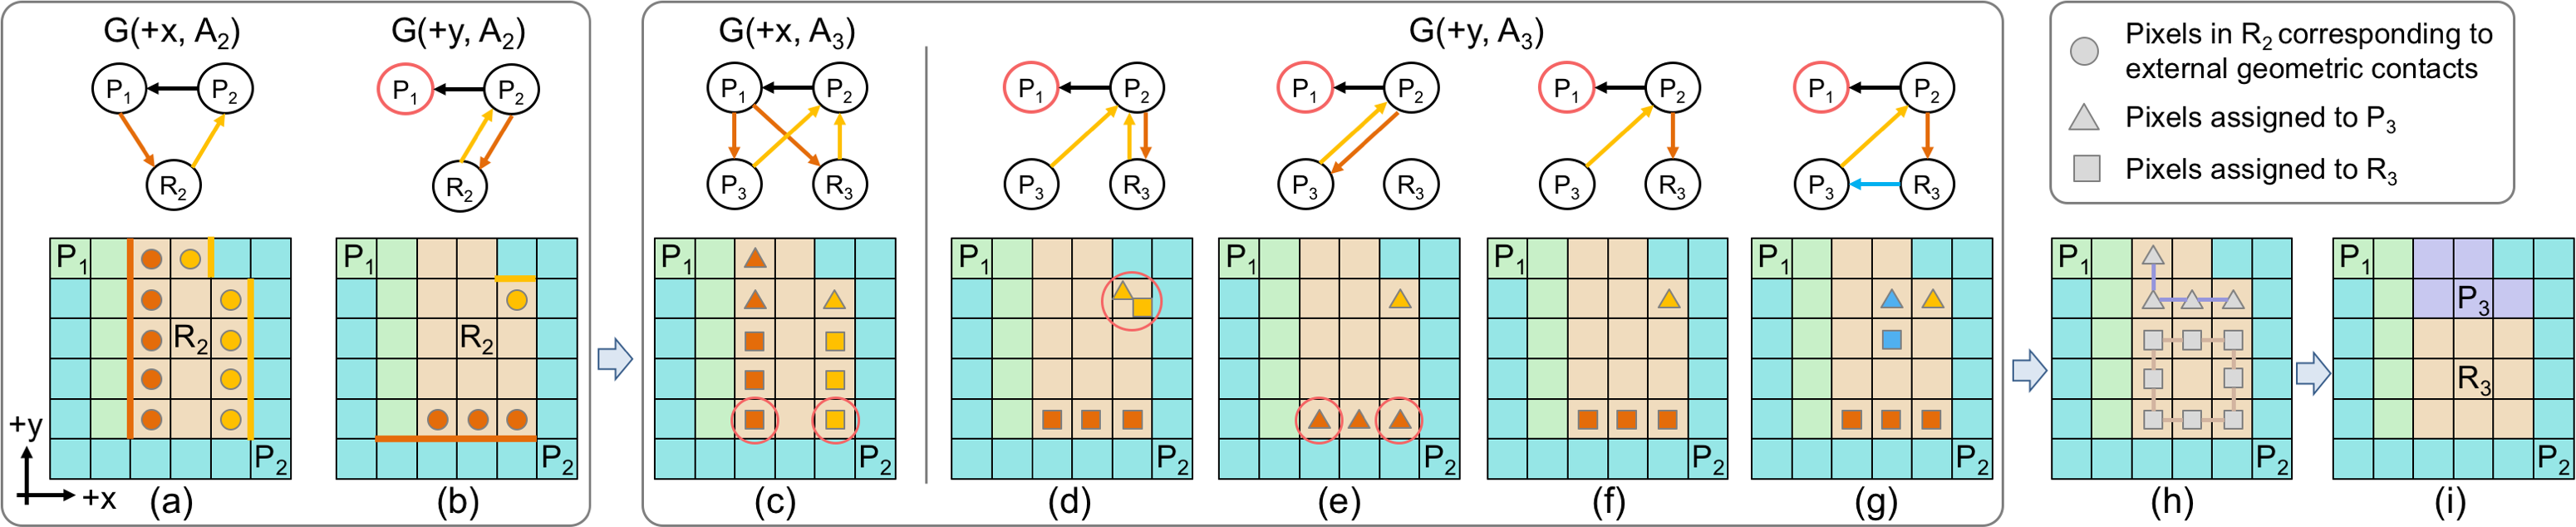
\includegraphics[width=17.80cm]{images/Framework_Geometry.png}
	\vspace*{-2.5mm}
	\caption{
		Geometry realization of $\{G(d, A_3)\}$.
		(a\&b) Identify geometric contacts between $\{P_1, P_2\}$ and $R_2$ in $\mathbf{A}_2$.
		(c-f) Distribute external geometric contacts between $P_3$ (shows as triangles) and $R_3$ (shown as squares) for (c) $G(+x, A_3)$ and (d-f) $G(+y, A_3)$,
		where (d\&e) show two failure examples.
		(g) Realize internal blocking relation between $P_3$ and $R_3$ in $G(+y, A_3)$.
		(h) Construct initial geometry of $P_3$ and $R_3$.
		(i) Resulting $\mathbf{A}_3$.
	}
	\vspace*{-2.0mm}
	\label{fig:Framework_Geometry}
\end{figure*}

\vspace*{-1.0mm}
Given these observations, we could find all valid graph designs by enumerating the distribution of external blocking relations, constructing the corresponding internal blocking relations, and testing the strongly connected property of the DBGs.
However, this generate-and-test approach could be very inefficient. The number of choices to distribute external blocking relations is $3^L$, where $L$ is the number of  edges of $R_{i-1}$ in $G(d, A_{i-1})$, since each edge of $R_{i-1}$ can be distributed to $P_i$, $R_i$, or both.
Figure~\ref{fig:Framework_Conceptual} shows an example with $3^2 =9$ graph designs, where $L=2$.



Rather than enumerating all possible graph designs, we propose an efficient approach to find a desired number of designs that are interlocking conceptually; see Figure~\ref{fig:Framework_Cycle}.
%\Mark{We need to be careful here. This statement suggest we look only at some subset of valid designs. Which subset is this? Are we not exploring the full search space?}
%\Peng{We are exploring the full search space since we can create blocking relation between $P_i$ and any other part (i.e., $\{P_1, ..., P_{i-1}\}$ and $R_i$) to immobilize $P_i$. The reason to find a few valid conceptual designs is due to the huge search space. 
%If we try to enumerate all of them, it is going to be a problem with exponential complexity. }
The key idea is to directly guarantee that each $G(d, A_i)$ is strongly connected by constructing a cycle in the graph that includes both $P_i$ and $R_i$, given that $G(d, A_{i-1})$ is already strongly connected.
%Denote the set of parts with an edge to (from) $R_{i-1}$ as $S_{in}$ ($S_{out}$).
Denote $S_{in}$ ($S_{out}$) as the set of parts with an edge to (from) $R_{i-1}$, and $P_{in}$ ($P_{out}$) as an arbitrary part in $S_{in}$ ($S_{out}$); see Figure~\ref{fig:Framework_Cycle}(a\&f).
According to the number of internal blocking relations to be constructed between $P_i$ and $R_i$ denoted as $K$,  we have the following three cases to construct the cycle that we can choose independently for each DBG. 
%\Mark{To the reader it might not be clear if these cases occur, or if we can arbitrarily choose any of the three.}
%\Peng{The motivation is to control the degree of connection strength by interlocking, depending on the users intent.
%We can either make an interlocking assembly with fewest number of blocking relations (case 3; easy to be realized but may not be steady) or with lots of redundant blocking relations (case 1 and 2; hard to be realized but more steady even during the intermediate assembly state). }

%analyze the edges of $R_{i-1}$ and search external blocking relations based on internal blocking relations between $P_i$ and $R_i$ to ensure that the base DBG is strongly connected.

\begin{enumerate}[label=(\arabic*), leftmargin=*]
	\vspace*{-0.5mm}
	\item
	{\em K=2.}  \
	$P_i \rightarrow  R_i \rightarrow  P_i$ forms a cycle, i.e., any distribution of external blocking relations works for this case; see Figure~\ref{fig:Framework_Cycle}(b).

	\vspace*{0.5mm}
	\item
	{\em K=1.} \
	$P_i \rightarrow  R_i \rightarrow  P_{out} \dashrightarrow P_{in} \rightarrow P_i$ ($R_i \rightarrow  P_i \rightarrow  P_{out} \dashrightarrow P_{in} \rightarrow R_i$) forms a cycle if the single directed edge is from $P_i$ to $R_i$ (from $R_i$ to $P_i$); see Figure~\ref{fig:Framework_Cycle}(c\&d).
    Here, $P_{out} \dashrightarrow P_{in}$ means that $P_{out}$ can reach $P_{in}$ in $G(d, A_{i-1})$ without passing through $R_{i-1}$, or $P_{out}$ and $P_{in}$ are the same part.

	\vspace*{0.5mm}
	\item
	{\em K=0.} \
	$P_i \rightarrow  P_{out} \dashrightarrow  P_{in} \rightarrow R_i \rightarrow  P_{out}^{'} \dashrightarrow P_{in}^{'} \rightarrow P_i$ forms a cycle, where $P_{in}$ and $P_{in}^{'}$ (as well as $P_{out}$ and $P_{out}^{'}$) are possible to be the same part; see Figure~\ref{fig:Framework_Cycle}(e).
	%In this case, no internal blocking relation needs to constructed since external blocking relations are sufficient to make the graph strongly connected; see Figure~\ref{fig:Framework_Conceptual}(d) rightmost for an example.
	
	%This is because fewer internal blocking relations provide more flexibility to construct the geometry of $P_i$ and $R_i$.	
\end{enumerate}	

Compared with case 1, cases 2 and 3 rely more on external blocking relations than on internal blocking relations to immobilize $P_i$ and $R_i$.
As a consequence, these two cases impose fewer constraints on the subsequent geometry construction of $P_i$ and $R_i$,  resulting in a higher chance to be successfully realized in the embedded geometry; compare the geometric examples in Figure~\ref{fig:Framework_Cycle}(g-j).

Besides interlocking, we also need to ensure that $P_i$ is disassemblable in $[P_i, R_i]$.
Thus, we require that $P_i$ and $R_i$ have fewer than two directed edges (i.e., case 2 and 3) in at least one base DBG.
The output of this stage is a set of $\{G(d, A_i)\}$ that satisfy the interlocking requirement, denoted as $\mathbf{C}_i$.

\if 0
Among all the generated conceptual designs, we prefer to select those that rely on more external blocking relations than internal blocking relations (i.e., above case 2 and 3) since these designs have fewer constraints on geometry construction of $P_i$ and $R_i$, resulting a higher chance to be successfully realized in the embedded geometry.
\fi





%\Peng{there are too many choices for the conceptual designs; how do we select good ones from them?}


%%%%%%%%%%%%%%%%%%%%%%%%%%%
% Geometry Realization of P_i and R_i
%%%%%%%%%%%%%%%%%%%%%%%%%%%

\begin{figure}[!b]
	\centering
	\vspace*{-3.5mm}
	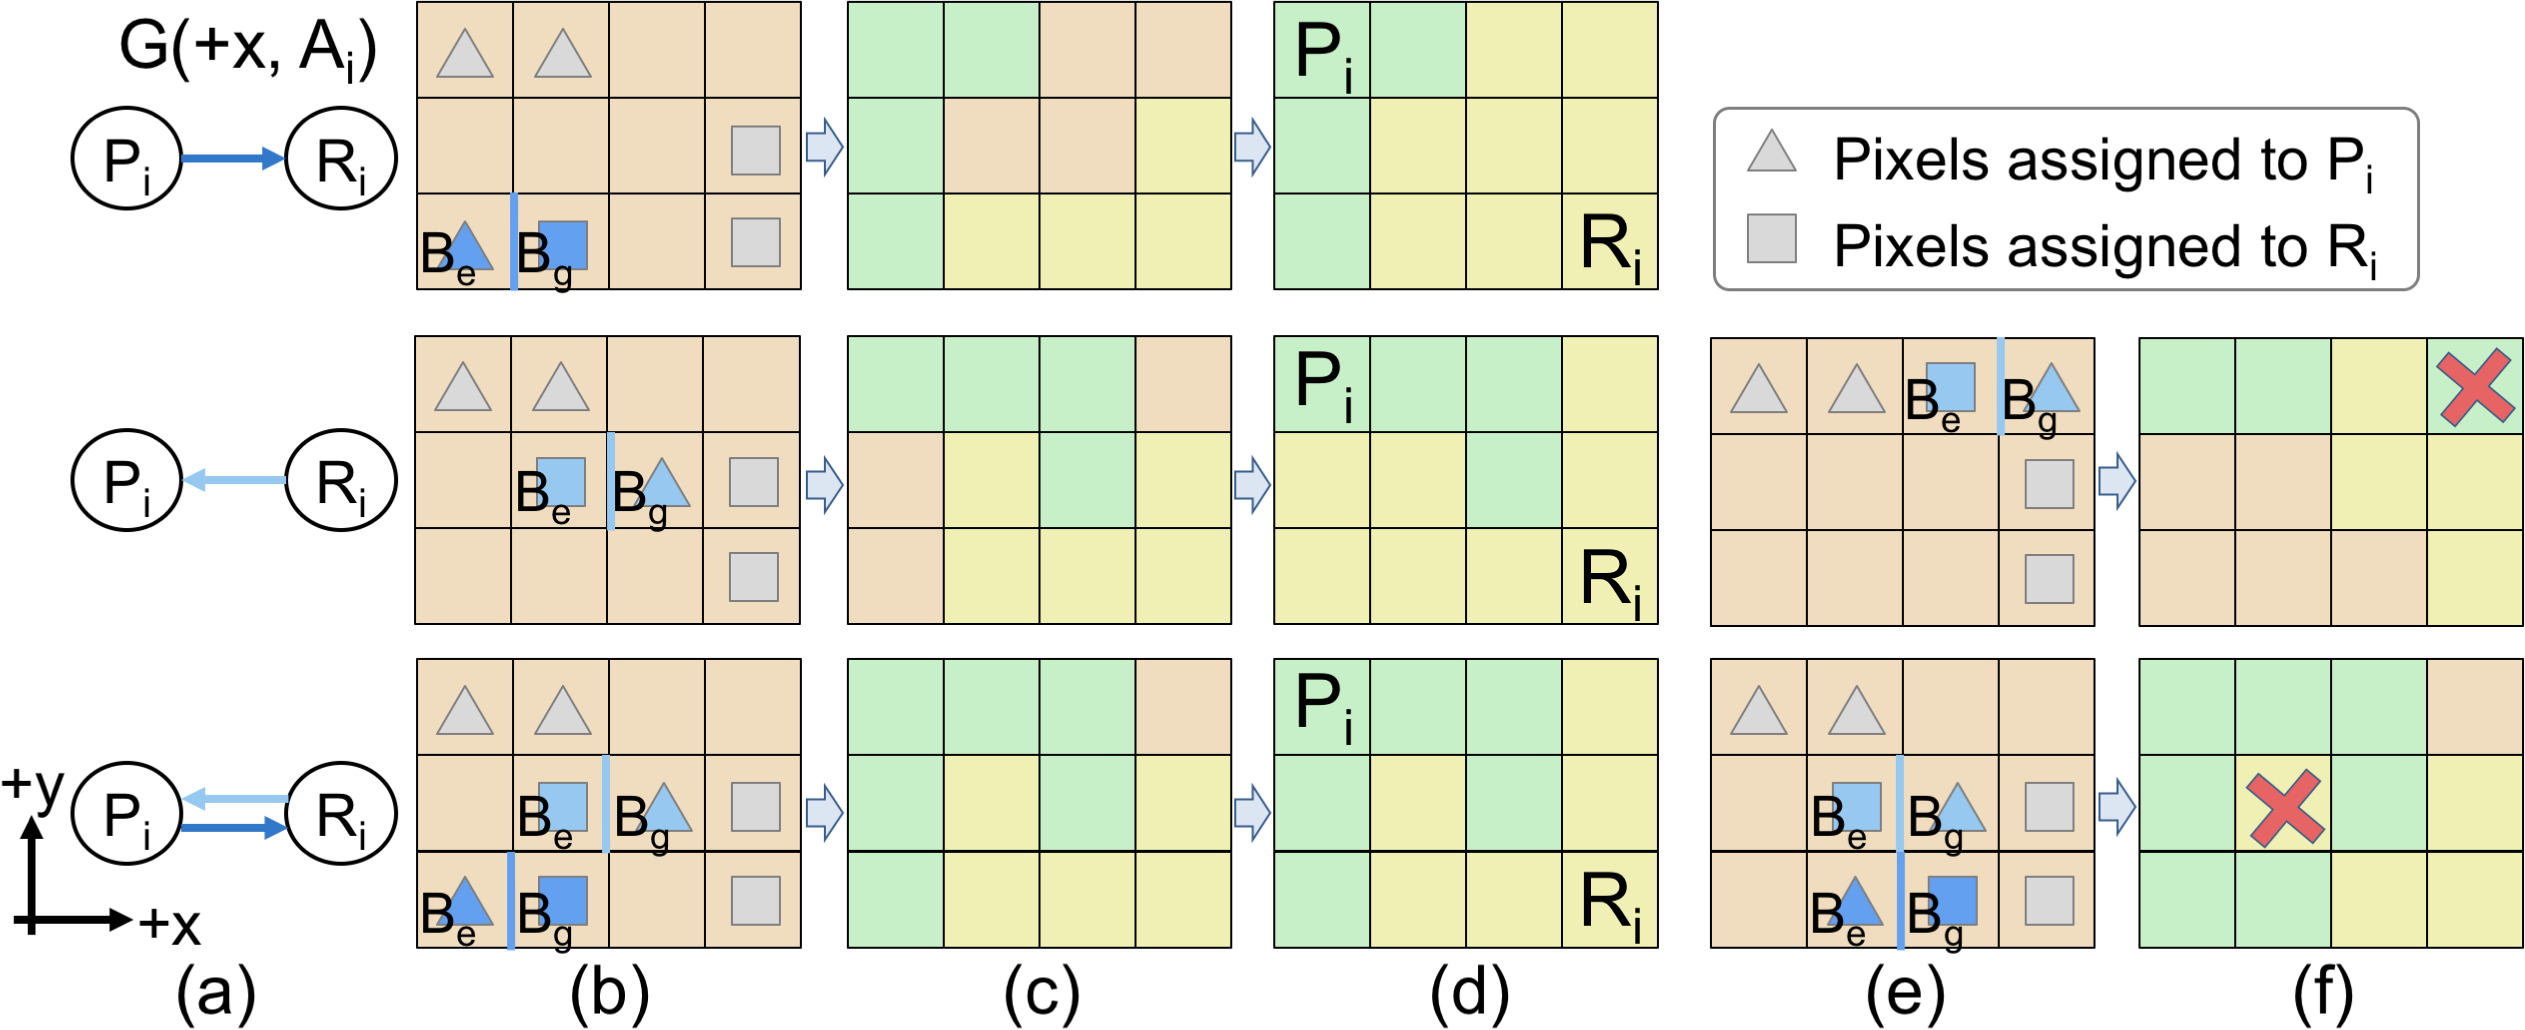
\includegraphics[width=8.45cm]{images/Framework_Blocking.png}
	\vspace*{-2.5mm}
	\caption{
		(a) Internal blocking relations between $P_i$ and $R_i$ in $G(+x, A_i)$.
		(b) Find blocking and blockee pixel in $R_{i-1}$ (in orange) according to the blocking relations.
		Blocking pixels and blockee pixels in (b) and their associated blocking relation in (a) are colored the same (light or dark blue).
		(c) Initial geometry of $P_i$ and $R_i$.
		(d) Final geometry of $P_i$ and $R_i$.
		(e\&f) Two failure examples due to disconnectivity of $P_i$ or $R_i$ (see the red cross).}
	%\vspace*{-4.5mm}
	\label{fig:Framework_Blocking}
\end{figure}

\begin{figure*}[!t]
	\centering
	%\vspace*{-3.5mm}
	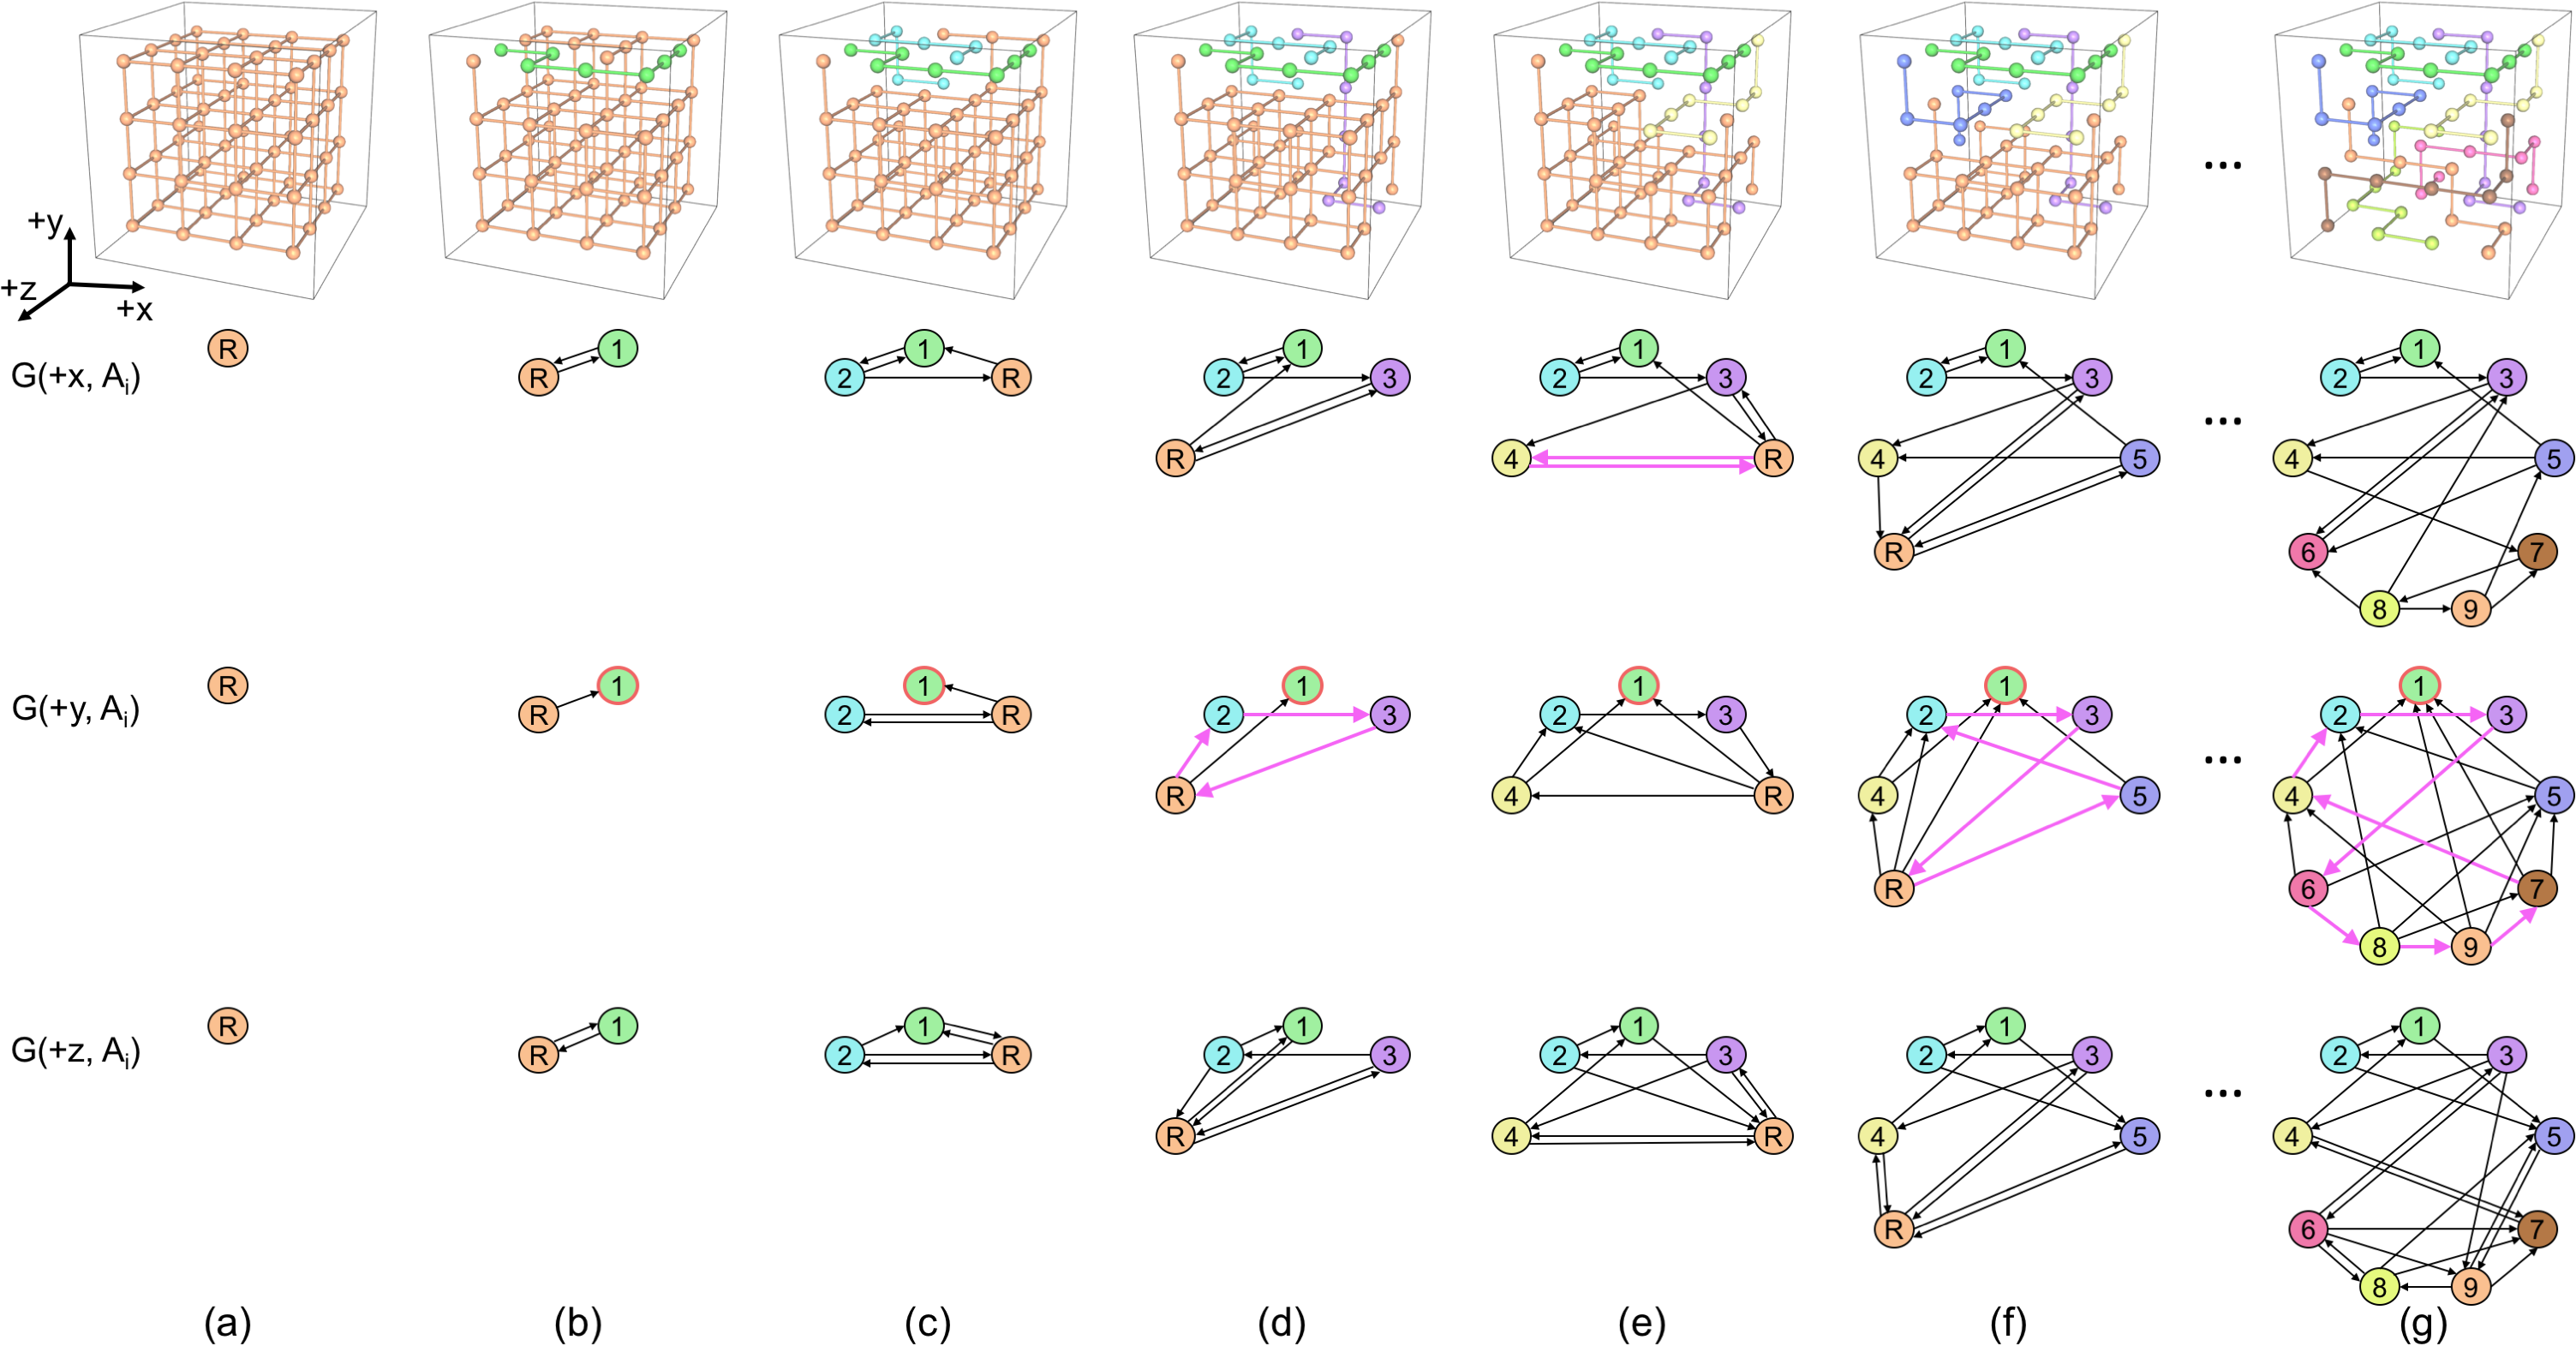
\includegraphics[width=17.7cm]{images/Application_Puzzle_Cube.png}
	\vspace*{-3.5mm}
	\caption{(a) Starting from a 4$\times$4$\times$4  voxel grid , (b-f) our framework iteratively construct the assembly pieces to create (g) a 9-piece interlocking {\textsc{Cube}}.
		Three DBGs are drawn for each intermediate assembly at the bottom.
		% where $P_i$ ($R_i$) are numbered as $i$ ($i+1$) in the DBGs. 
		Our approach allows immobilizing $P_i$ and $R_i$ by constructing cycles of various sizes (examples colored in purple).
		%The number of edges in the DBGs of~\cite{Song-2012-InterCubes} (21, 19, and 19, from top to bottom) is larger than (n) those of ours (14, 18, and 16, from top to bottom).	
		%This is because our approach allows constructing larger cycles to immobilize $P_i$ and $R_i$ (compare the cycles colored in purple in (d\&k) and (g\&n)).
		%The cycles (colored in purple) constructed to immobilize $P_4$ and $R_4$ have (d) 3 and (k) 4 parts respectively while those to immobilize $P_7$ and $R_7$ have (d) 3 and (k) 6 parts respectively.
	}
	\vspace*{-2.0mm}
	\label{fig:Application_Puzzle_Cube}
\end{figure*}


\vspace*{1.0mm}
\noindent
{\bf Geometry Realization of $P_i$ and $R_i$.}  \
%Now, a conceptual design of $P_i$ and $R_i$ has been represented as  a set of new directed edges in the base DBGs $\{G(d, A_i)\}$.
In order to realize $\{G(d, A_i)\}$ $\in \mathbf{C}_i$ in the embedded geometry, 
we perform the following steps, each corresponding to a counterpart of the graph design stage:
%, which can be customized for designing different kinds of interlocking assemblies.
%Here, we take 2D interlocking puzzle design as an example for illustration.
%\Mark{describe the correspondence between conceptual design and geometric realization}

\vspace*{1.0mm}
\noindent
{\em i) Identify external geometric contacts between $\{P_1, ..., P_{i-1}\}$ and $R_{i-1}$. } \
Recall that a directed edge $e_{i \rightarrow j}$ from $P_i$ to $P_j$ in $G(d, A)$ means that $P_j$ blocks the translation of $P_i$ along $d$.
This indicates that $P_i$ contacts $P_j$ along $d$, and $P_j$ locates further than $P_i$ along $d$; see again Figure~\ref{fig:NDBG}.
In an assembly $\mathbf{A}_{i-1}$, we identify such blocking contacts between $P_l$ ($1\leq l\leq{i-1}$) and $R_{i-1}$ for each base direction $d$ by computing the overlap of the respective boundaries along $d$ ($-d$), see Figure~\ref{fig:Framework_Geometry}(a\&b).



\vspace*{1.0mm}
\noindent
{\em ii) Distribute external geometric contacts. } \
An external blocking relation, say between $P_l$ and $R_{i-1}$,  in a DBG $G(d, A_{i-1})$ can be distributed to $P_i$, $R_i$, or both.
For the first two cases, the corresponding geometric contacts need to be totally assigned to $P_i$ or $R_i$ respectively; see Figure~\ref{fig:Framework_Geometry}(f).
For the last case, the geometric contacts need to be partitioned into two subsets and assigned to $P_i$ and $R_i$ separately; see Figure~\ref{fig:Framework_Geometry}(c).

However, this step could fail for two reasons.
First, the external geometric contact could be too small to be partitioned.
For example, $R_2$ contacts $P_2$ along $+y$ in a single pixel in Figure~\ref{fig:Framework_Geometry} (b).
Yet, this single pixel (marked with a red circle) needs to be assigned to both $P_3$ and $R_3$ in Figure~\ref{fig:Framework_Geometry}(d) according to the computed blocking relations, which is not feasible.
Second, the assignment of geometric contacts may conflict with one another across multiple DBGs.
For example, two pixels marked with red circles in Figure~\ref{fig:Framework_Geometry}(c) need to be assigned to $R_3$ to realize $G(+x, A_3)$.
However, these two pixels also need to be assigned to $P_3$ to realize $G(+y, A_3)$ in Figure~\ref{fig:Framework_Geometry}(e), leading to a conflict. 
 
\vspace*{1.0mm}
\noindent
{\em iii) Construct internal geometric contacts. } \
If $G(d, A_i)$ has $K\in \{1, 2\}$ internal blocking relations, we need to construct geometric contacts between $P_i$ and $R_i$.
Here, we take as an example the case of realizing a single directed edge from $P_i$ to $R_i$ to illustrate our approach; see Figure~\ref{fig:Framework_Blocking}(top).
Inspired by~\cite{Song-2012-InterCubes}, we find a pair of blocking and blockee pixels denoted as $B_g$ and $B_e$, respectively, which contact each other along $d$ among all unassigned pixels in $R_{i-1}$.
We then assign $B_e$ to $P_i$ and $B_g$ to $R_i$.
Other cases of realizing internal blocking relations can be handled similarly; see Figure~\ref{fig:Framework_Blocking}.

%Note that this step also could fail since we may not be able to find such a pair of blocking and blockee voxels, and/or the assignments of blocking and blockee voxels may make $[P_i, R_i]$ deadlocking or $R_i$ disconnected; see Figure~\ref{fig:Framework_Geometry}(d).

%There are generally four cases of creating internal blocking relations between $P_i$ and $R_i$ along $d$; see Figure~\ref{fig:Blocking_Relation}.

\vspace*{1.0mm}
\noindent
{\em iv) Construct initial parts geometry. } \
By now, we have identified all the pixels in $R_{i-1}$ that need to be assigned to $P_i$ or $R_i$ to make $\mathbf{A}_i$ interlocking.
%We further identify all pixels on top of $P_i$ along $d$ to $P_i$ such that $P_i$ is separable from $R_i$ in $[P_i, R_i]$ along $d$; see the pixel with a pink marker in Figure~\ref{fig:Framework_Geometry}(h).
To form an initial $P_i$ ($R_i$), we connect these pixels into a single part using the shortest path; see Figure~\ref{fig:Framework_Geometry}(h) and~\ref{fig:Framework_Blocking}(c).
Note that this connection process can fail since we may not be able to find such a shortest path without disconnecting parts; see Figure~\ref{fig:Framework_Blocking}(e\&f) for examples.

\vspace*{1.0mm}
\noindent
{\em v) Ensure disassemblability. } \
To make $P_i$ movable in $[P_i, R_i]$, we first identify all possible moving directions of $P_i$ in $\{G(d, A_i)\}$, i.e., the directions where $P_i$ is unblocked by $R_i$; e.g.,  $P_3$ could be movable along $\{-x, +x, +y\}$ in $[P_i, R_i]$ according to the blocking graph in Figure~\ref{fig:Framework_Geometry}(c\&g) .
We try each possible moving direction of the initial $P_i$ and discard those that cannot be achieved in the embedded geometry. 
%e.g., $P_i$ seems movable along $+x$ in Figure~\ref{fig:Framework_Blocking}(middle; a) according to the conceptual design yet it cannot really move along $+x$ due to blocking of $R_i$ in Figure~\ref{fig:Framework_Blocking}(middle; b\&c).
We consider that $P_i$ is disassemblable in $[P_i, R_i]$ if we can find one movable direction of $P_i$, along with a disassembly path.
Lastly, we assign those remaining pixels in $R_{i-1}$ (see orange pixels in Figure~\ref{fig:Framework_Blocking}(c)) to $P_i$ and $R_i$ respectively according to geometric proximity (with preference to $R_i$), while maintaining the disassemblability of $P_i$ in $[P_i, R_i]$; see Figure~\ref{fig:Framework_Geometry}(i) and~\ref{fig:Framework_Blocking}(d).

A graph design is realized if all above steps succeed. Otherwise, we discard this design and try another one in $\mathbf{C}_i$. If all candidates in $\mathbf{C}_i$ fail, we backtrack to the other nodes in the construction tree following the procedure in Algorithm~\ref{alg:Alg_Framework}.


%\Mark{In the above paragraphs and figures, we frequently mention failure case, but we do not state how we handle them. We should state very clearly what happens if one step fails!}

%\Mark{In general, the above explanation is very descriptive, i.e. it explains the steps of the algorithm, but it does not necessarily explain, why this is the only/right approach to take. It might help to have a high-level overiew, maybe some pseudo-code or diagram, to provide a big-picture view of the method.}

%\Mark{It might also not be clear how representative the puzzle example is. It's good to explain the algorithm, but is it obvious how other cases are treated, i.e. will readers understand that this in indeed a general approach? Maybe a forward reference to the next section would be helpful.}

%Note that this step also could fail since the assignment of voxels could make $[P_i, R_i]$ deadlocking and/or or $R_i$ and/or disconnected; see Figure~\ref{fig:Framework_Geometry}(d).

%This is achieved by properly assigning remaining geometry in $R_{i-1}$ to $P_i$ or $R_i$; see Figure~\ref{fig:Framework_Geometry}(i) for an example. %\Peng{may need more details here.}



%%%%%%%%%%%%%%%%%%%%%%%%%%%%%%%%%%%%%%%%%%%%%%%%%%%%%%%%%%%%%%%%%%%%%%%%%%%%%%%%%%%%%%%%%%%%%%%%%%%
% Backup
%%%%%%%%%%%%%%%%%%%%%%%%%%%%%%%%%%%%%%%%%%%%%%%%%%%%%%%%%%%%%%%%%%%%%%%%%%%%%%%%%%%%%%%%%%%%%%%%%%%








